\section{Six point comparison}

\begin{thm}{Theorem}
Any Alexandrov space with nonnegative curvature satisfies the tree comparison for the following two trees:

\begin{comment}
\begin{center}
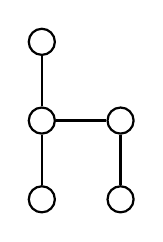
\begin{tikzpicture}[scale=1,
  thick,main node/.style={circle,draw,font=\sffamily\bfseries,minimum size=3mm}]
  \node[main node] (1) at (0,0) {};
  \node[main node] (2) at (0,1){};
  \node[main node] (3) at (0,2){};
  \node[main node] (4) at (1,0) {};
  \node[main node] (5) at (1,1) {};
  

  \path[every node/.style={font=\sffamily\small}]
   (1) edge node[above]{}(2)
   (2) edge node[above]{}(3)
   (2) edge node[above]{}(5)
   (4) edge node[above]{}(5);
\end{tikzpicture}
\hskip10mm
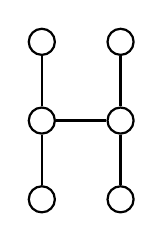
\begin{tikzpicture}[scale=1,
  thick,main node/.style={circle,draw,font=\sffamily\bfseries,minimum size=3mm}]

  \node[main node] (1) at (0,0) {};
  \node[main node] (2) at (0,1){};
  \node[main node] (3) at (0,2){};
  \node[main node] (4) at (1,0) {};
  \node[main node] (5) at (1,1) {};
  \node[main node] (6) at (1,2) {};

  \path[every node/.style={font=\sffamily\small}]
   (1) edge node[above]{}(2)
   (2) edge node[above]{}(3)
   (2) edge node[above]{}(5)
   (4) edge node[above]{}(5)
   (5) edge node[above]{}(6);
\end{tikzpicture}
\hskip10mm
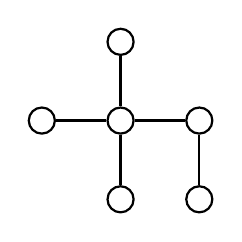
\begin{tikzpicture}[scale=1,
  thick,main node/.style={circle,draw,font=\sffamily\bfseries,minimum size=3mm}]

  \node[main node] (1) at (0,1) {};
  \node[main node] (2) at (1,0){};
  \node[main node] (3) at (1,1){};
  \node[main node] (4) at (1,2) {};
  \node[main node] (5) at (2,0) {};
  \node[main node] (6) at (2,1) {};

  \path[every node/.style={font=\sffamily\small}]
   (1) edge node[above]{}(3)
   (2) edge node[above]{}(3)
   (3) edge node[above]{}(6)
   (4) edge node[above]{}(3)
   (5) edge node[above]{}(6);
\end{tikzpicture}
\end{center}
\end{comment}

\end{thm}

\parbf{Pivotal configurations.}
Let $T$ be a dipolar tree.
Label the poles of $T$ by $p_1$ and $p_2$ and the reaming vertexes by $x_1,x_2,\dots,x_n$.

A point array $p_1,p_2,x_1,\dots x_n\in A$ together with choice one geodesic connecting adjacent vertexes of $T$ will be called \emph{geodesic $T$-tree};
it contains one geodesic $[p_1,p_2]$ and $n$ geodesics  $[p_i,x_j]$.

A model configuration $\~p_1$, $\~p_2$, $\~x_1,\dots\~x_n\in \RR^n$ will be called \emph{pivotal configuration} of the geodesic $T$-tree in $A$
if 
\begin{enumerate}[(i)]
\item $|\~p_1-\~p_2|= |p_1-p_2|$,
\item $|\~p_i-\~x_j|= |p_i-p_j|$ for any edge $p_ix_j$ in $T$ and
\item $\measuredangle[\~p_j\,^{\~x_k}_{\~p_i}]_{\RR^n}=\measuredangle[\~p_j\,^{\~x_k}_{\~p_i}]_A$
for any hinge  $[p_j\,^{x_k}_{\~p_i}]$ in $T$.
\end{enumerate}

Note that by angle comparison 
\[|\~x_i-\~p_j|_{\RR^n}\ge |x_i-p_j|_A\]
for any $i$ and $j$.
Therefore, in order to check that a pivotal configuration $\~p_1$, $\~p_2$, $\~x_1,\dots\~x_n\in \RR^n$ satisfies the conditions in the $T$-tree comparison (see Section~\ref{sec:intro}) it is sufficient to check that 
\[|\~x_i-\~x_j|_{\RR^n}\ge |x_i-x_j|_A\]
for all $i,j$.

Up to a motion of $\RR^n$, a pivotal configuration is completely described by the angles $\alpha_{i,j}$ between the half-planes passing $\~x_i$ and $\~x_j$ with $\~p_1 \~p_2$ as the the boundary line.

Let us denote by $\beta_{i,j}$ the minimal angle between the planes $\~p_1 \~p_2 \~x_i$ and $p_1p_2 x_j$ in a pivotal configuration such that $|\~x_i-\~x_j|_{\RR^3}\ge|\~x_i-\~x_j|_A$. 
Note that a pivotal  configuration $\~p_1,\~p_2,\~x_1,\dots,\~x_n$ satisfies the conditions in the definition of comparison if and only if $\alpha_{i,j}\ge \beta_{i,j}$ for all pairs $(i,j)$.


\begin{thm}{Lemma}\label{|x-x|}
For any dipolar tree as above we have 
\[\beta_{i,j}\le \pi\]
for any pair $i$ and $j$.

In other words, for any broken geodesic line $x_1p_1p_2x_2$ in a nonnegatively curved Alexandrov space $A$ there is a pivotal configuaration $\~p_1,\~p_2,\~x_1,\~x_2\in \RR^2$ such that 
\[|\~x_1-\~x_2|_{\RR^2}\ge |x_1-x_2|_A.\]

\end{thm}

\parit{Proof.}
Consider the pivotal configuaration $\~p_1\~p_2\~x_1\~x_2\in \RR^2$ such that $\~x_1$ and $\~x_2$ lie on the opposite sides from the line $\~p_1\~p_2$.
Note that the line segment $[\~x_1,\~x_2]$ intersects the line $\~p_1\~p_2$;
denote by $\~z$ the point of intersection.

If $\~z\in [\~p_1,\~p_2]$, consider the corresponding point $z\in [p_1,p_2]$.
In the remaining case, $\~z\notin [\~p_1,\~p_2]$, without loss of generality, we can assume that $\~z$ lies on the half line starting at $\~p_1$.
In this case set $z$ to be the image of $p_2$ for the $(\tfrac12\cdot \dist_{p_1}^2)$-gradient flow of $p_2$ for time $t=\ln \tfrac{|\~z-\~p_1|}{|\~p_2-\~p_1|}$.
In both cases the comparsison implies 
\begin{align*}
|x_i-z|_A &\le |\~x_i-\~z|_{\RR^2},
&
|x_j-z|_A &\le |\~x_j-\~z|_{\RR^2}.
\end{align*}
From the triangle inequality, the lemma follows.
\qeds

The following lemma is proved along the same lines.

\begin{thm}{Lemma}
For any dipolar tree as above we have 
\[\beta_{i,j}+\beta_{j,k}+\beta_{k,i}\le 2\cdot\pi.\]
for any triple $i$, $j$ and $k$.

In other words, for any geodesic (2-1)-tree $x_1p_1p_2x_2$ in a nonnegatively curved Alexandrov space $A$ there is a pivotal configuaration $\~p_1,\~p_2,\~x_1,\~x_2,x_3\in \RR^3$ such that 
\begin{align*}
|\~x_1-\~x_2|_{\RR^2}&\ge |x_1-x_2|_A,
\\
|\~x_2-\~x_3|_{\RR^2}&\ge |x_2-x_3|_A,
\\
|\~x_3-\~x_1|_{\RR^2}&\ge |x_3-x_1|_A.
\end{align*}



\end{thm}



\parit{Proof.}
Assume contrary; that is 
\[\beta_{i,j}+\beta_{j,k}+\beta_{k,i}> 2\cdot\pi.\eqlbl{eq>2pi}\]
Since $\beta_{i,k}\le \pi$, it follows that 
\[\beta_{i,j}+\beta_{j,k}> \pi.\eqlbl{sum>=pi}\] 
Consider the pivotal configuration $\~p_1,\~p_2,\~x_i,\~x_j,\~x_k\in\RR^3$ such that 
$\alpha_{i,j}=\beta_{i,j}$, $\alpha_{j,k}=\beta_{j,k}$ and the points $\~x_i$ and $\~x_k$ lie on the opposite sides from the plane $\~p_1\~p_2\~x_j$.
By \ref{sum>=pi}, $[\~x_i\~x_j\~x_k]$ intersects the line $\~p_1\~p_2$;
denote by $\~z$ the point of intersection.

Let us construct a point $z\in A$ which corresponds to $\~z$ the same way as in the proof of Lemma~\ref{|x-x|}.
By construction, 
\begin{align*}
|x_i-x_j|_A &= |\~x_i-\~x_j|_{\RR^3},
&
|x_j-x_k|_A &= |\~x_j-\~x_k|_{\RR^3}.
\end{align*}
From \ref{eq>2pi},
\[|x_i-x_k|_A > |\~x_i-\~x_k|_{\RR^3}\]
By comparison
\begin{align*}
|x_i-z|_A &\le |\~x_i-\~z|_{\RR^3},
&
|x_j-z|_A &\le |\~x_j-\~z|_{\RR^3},
&
|x_k-z|_A &\le |\~x_k-\~z|_{\RR^3}.
\end{align*}
Which leads to a contradiction. %???
\qeds


Assume one of the triangle inequalities 
\[\beta_{i,k}\le \beta_{i,j}+\beta_{j,k}\]
does not hold.
Order the values $\{\beta_{i,j}\}$ in a nonincreasing order.
Let us construct a metric graph with 4 vertexes labeled by $\{1,2,3,4\}$
the following way choose the the largest value $\beta_{i,j}$ 
and attche an edge $(i,j)$ of length $\beta_{i,j}$,
do the same for the second largest value and so on,
starting from third step, before adding new edge we have to check that the triangle inequalities does not brake; in other words we want to 
At the end we get a metric 
\qeds
